\documentclass[12pt]{letter}
\usepackage{amsmath,amsfonts,amsthm,amstext,amssymb,graphicx, multicol,fancyhdr,lastpage,fullpage,framed,fancybox,enumerate,tikz,color,mathrsfs, polynom, pifont, stmaryrd}
\usepackage[margin=0.6in,headsep=3pt, headheight=15pt]{geometry}

% ----------------------------------------------------------
% Custom Definitions, Commands, Environments, etc.

% Sets of numbers
\def\R{\mathbb{R}} % The reals
\def\N{\mathbb{N}} % The naturals
\def\Z{\mathbb{Z}} % The integers
\def\Q{\mathbb{Q}} % The rationals

% Blank space
\newcommand{\blank}[1]{\underline{\hspace{#1}}} % Blank space

% Change font colors
\newcommand{\cyan}[1]{{\color{cyan}{#1}}} % Changes font to cyan
\newcommand{\red}[1]{{\color{red}{#1}}} % Changes font to red
\newcommand{\magenta}[1]{{\color{magenta}{#1}}} % Changes font to magenta
\newcommand{\orange}[1]{{\color{orange}{#1}}} % Changes font to orange
\newcommand{\yellow}[1]{{\color{yellow}{#1}}} % Changes font to yellow
\newcommand{\violet}[1]{{\color{violet}{#1}}} % Changes font to violet
\newcommand{\green}[1]{{\color{green}{#1}}} % Changes font to green
\newcommand{\blue}[1]{{\color{blue}{#1}}} % Changes font to blue
\newcommand{\white}[1]{{\color{white}{#1}}} % Changes font to white

% Fitted inclusion symbols
\newcommand{\fp}[1]{\left({#1}\right)} % Fitted parentheses around content
\newcommand{\fb}[1]{\left[{#1}\right]} % Fitted brackets
\newcommand{\lhoi}[1]{\left({#1}\right]} % Left half-open interval
\newcommand{\rhoi}[1]{\left[{#1}\right)} % Right half-open interval
\newcommand{\set}[1]{\left\{{#1}\right\}} % Fitted braces (useful for sets)
\newcommand{\av}[1]{\left|{#1}\right|} % Fitted absolute value bars
\newcommand{\step}[1]{\left\llbracket {#1} \right\rrbracket}

% Augmented Matrix Environment
\newenvironment{amatrix}[1]{%
	\left[\begin{array}{@{}*{#1}{c}|c@{}}
	}{%
	\end{array}\right]
}

% Miscellaneous
\def\then{\Rightarrow}
\def\to{\rightarrow}
\def\d{^{\circ}}
\newcommand{\?}{\stackrel{?}{=}}
\newcommand{\cmark}{\text{ \ding{51}}}
\newcommand{\xmark}{\text{ \ding{55}}}



% Coordinate Plane (Four-Quadrant)
\def\coordplane {
	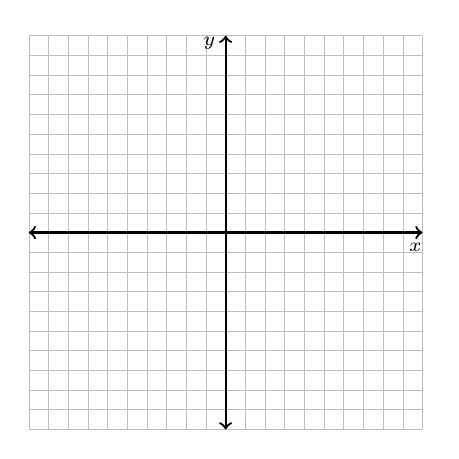
\begin{tikzpicture}        \draw[step=0.25cm,black,very thin,opacity=0.25] (-2.5cm, -2.5cm) grid (2.5cm, 2.5cm);
	\draw[<->,thick,black] (-2.5cm, 0) -- (2.5cm, 0) node[anchor=north west,pos=0.94,font=\scriptsize]{$x$};
	\draw[<->,thick,black] (0,-2.5cm) -- (0, 2.5cm) node[anchor=south east,font=\scriptsize,pos=0.94]{$y$};
	\end{tikzpicture}
}

% Coordinate Plane (One-Quadrant)
\def\onequad {
	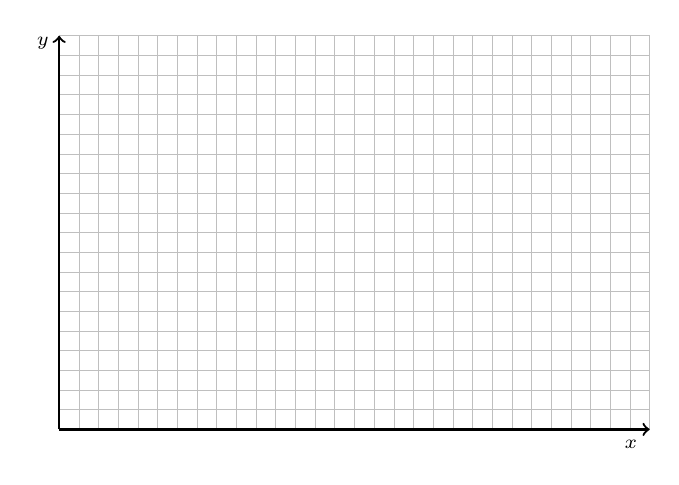
\begin{tikzpicture}
	\draw[step=0.25cm, black, very thin, opacity=0.25] (0,0) grid (7.5cm,5cm);
	\draw[->, thick, black] (0,0) -- (7.5cm, 0) node[anchor=north west,font=\scriptsize,pos=0.94]{$x$};
	\draw[->, black, thick] (0,0) -- (0,5cm) node[anchor=south east,font=\scriptsize,pos=0.94]{$y$};
	\end{tikzpicture}
}

% Counters
\newcounter{exercise}

% Exercise environment (auto-numbered)
\newenvironment{exercise}[1][]{\begin{framed}\refstepcounter{exercise}\textbf{Exercise~\theexercise:} #1}{\end{framed}}

% Book exercise environment
\newenvironment{bex}[2] {
	\begin{framed}
		\textbf{Book Exercise {#1}:} #2
	\end{framed}	
}
% ----------------------------------------------------------

% ----------------------------------------------------------
% Header and Footer Information
% \pagestyle{fancy}
% \fancyhf{}
% \renewcommand{\headrulewidth}{0pt}
% \rhead{Name: \blank{2in}}
% \lhead{@}
% \rfoot{Page \thepage \, of \,\pageref{LastPage}}
% ----------------------------------------------------------
\author{Jacob Ayers}

\begin{document}

\textbf{Midterm 1 \\ MAT 130}
	
Please do not write on this test document. All work should be done on blank scratch paper, and all answers should be written on your answer document. Read all instructions before you begin.

\textbf{Instructions:} Complete each exercise to the best of your ability. Each exercise has exactly one correct answer, and worth four points. There is no partial credit available. You must complete this exam during class time, so keep a close eye on the clock. You may use the following materials on this exam: \begin{itemize}
	\item Pencil
	\item Unlimited blank scratch paper (provided by proctor)
	\item One page (8.5" x 11"; front/back) notes
	\item Graphing Calculator (not a phone calculator)
	\item GeoGebra Classic (web or desktop software; not on a phone)
\end{itemize}
Use of any other resources or materials is prohibited. If you are found to be using a prohibited resource or material, this exam will be scored as a zero. Good luck!

\begin{exercise}
	Evaluate $x^2 + 7x -3$ when $x = -3$. \begin{enumerate}[A.]
		\item $-15$
		\item $27$
		\item $0$
		\item $-33$
	\end{enumerate}
\end{exercise}

% My answer here


\vfill % \newpage

\begin{exercise}
	Simplify the expression $\fp{4a}^3\fp{5a^2}$. \begin{enumerate}[A.]
		\item $320a^6$
		\item $20a^5$
		\item $320a^5$
		\item $20a^6$
	\end{enumerate}
\end{exercise}

% My answer here


\vfill % \newpage

\begin{exercise}
	Find the product: $\fp{2x - 3}^2$. \begin{enumerate}[A.]
		\item $4x^2 - 12x + 9$
		\item $4x^2 + 9$
		\item $4x^2 + 12x + 9$
		\item $2x^2 - 6x + 9$
	\end{enumerate}
\end{exercise}

% My answer here


\vfill \newpage

\begin{exercise}
	Factor completely: $27x^3 - 8$. \begin{enumerate}[A.]
		\item $(3x + 2)(3x-2)$
		\item $(3x - 2)^3$
		\item $(3x + 2)\fp{9x^2 - 6x + 4}$
		\item $\fp{3x - 2}\fp{9x^2 + 6x + 4}$
	\end{enumerate}
\end{exercise}

% My answer here


\vfill % \newpage

\begin{exercise}
	Find the domain of the expression: $\sqrt{x - 8}$. \begin{enumerate}[A.]
		\item $[-8, \infty)$
		\item $[8, \infty)$
		\item $(-\infty, 8]$
		\item $(-\infty, -8]$
	\end{enumerate}
\end{exercise}

% My answer here


\vfill % \newpage

\begin{exercise}
	Perform the operation and simplify: $\dfrac{x^2 - 7x + 12}{x^2 + 8x + 16} \cdot \dfrac{x + 4}{x^2 - 9}$ \begin{enumerate}[A.]
		\item $\dfrac{1}{(x+4)(x+3)}$
		\item $\dfrac{x-4}{(x+4)(x+3)}$
		\item $x - 4$
		\item $\dfrac{x+4}{(x-4)(x+3)}$
	\end{enumerate}
\end{exercise}

% My answer here


\vfill % \newpage

\begin{exercise}
	To the nearest hundredth, find the distance between $\fp{-3.5, 6.1}$ and $\fp{2.8, 9.9}$. \begin{enumerate}[A.]
		\item $8.41$
		\item $3.86$
		\item $7.36$
		\item $16.02$
	\end{enumerate}
\end{exercise}

% My answer here


\vfill \newpage

\begin{exercise}
	Test the equation $y = \av{x} - 4$ for symmetry about both axes. \begin{enumerate}[A.]
		\item Symmetric about both the $x$-axis and the $y$-axis
		\item Symmetric about neither the $x$-axis nor the $y$-axis
		\item Symmetric about the $x$-axis
		\item Symmetric about the $y$-axis
	\end{enumerate}
\end{exercise}

% My answer here


\vfill % \newpage

\begin{exercise}
	Solve for $x$: $\dfrac{x}{4} - 5 = \dfrac{x}{5} + 6$. \begin{enumerate}[A.]
		\item $240$
		\item $180$
		\item $200$
		\item $220$
	\end{enumerate}
\end{exercise}

% My answer here


\vfill % \newpage

\begin{exercise}
	Which of the following is the $x$-intercept of the equation $3x + 8y = 48$? \begin{enumerate}[A.]
		\item $(16, 0)$
		\item $(0, 16)$
		\item $(6, 0)$
		\item $(0, 6)$
	\end{enumerate}
\end{exercise}

% My answer here


\vfill % \newpage

\begin{exercise}
	Solve for $r$: $V = \pi r^2 h$ \begin{enumerate}[A.]
		\item $r = \fp{\dfrac{V}{\pi h}}^2$
		\item $r = \sqrt{\dfrac{V}{\pi h}}$
		\item $r = \fp{\pi h V}^2$
		\item $r = \sqrt{\pi h V}$
	\end{enumerate}
\end{exercise}

% My answer here


\vfill \newpage

\begin{exercise}
	Solve for $x$: $-2x^2 - 5x + 27 = 0$ \begin{enumerate}[A.]
		\item $x = \dfrac{-5 \pm \sqrt{241}}{2}$
		\item $x = \dfrac{5 \pm \sqrt{241}}{2}$
		\item $x = \dfrac{5 \pm \sqrt{241}}{4}$
		\item $x = \dfrac{-5 \pm \sqrt{241}}{4}$
	\end{enumerate}
\end{exercise}

% My answer here


\vfill % \newpage

\begin{exercise}
	Write the quotient in standard form: $\dfrac{4 - 3i}{2 + 5i}$ \begin{enumerate}[A.]
		\item $\dfrac{23}{21} + \dfrac{26}{21}i$
		\item $\dfrac13 + \dfrac{26}{21}i$
		\item $-\dfrac{7}{29}-\dfrac{26}{29}i$
		\item $\dfrac{23}{29} - \dfrac{26}{29}i$
	\end{enumerate}
\end{exercise}

% My answer here


\vfill % \newpage

\begin{exercise}
	Which of the following is NOT a solution to the equation $x^3 - 7x^2 + 4x - 28 = 0$? \begin{enumerate}[A.]
		\item $-2i$
		\item $2i$
		\item $-7$
		\item $7$
	\end{enumerate}
\end{exercise}

% My answer here


\vfill % \newpage

\begin{exercise}
	Solve for $x$: $-3\fp{x - 5} \leq 4x - 13$ \begin{enumerate}[A.]
		\item $x \geq 4$
		\item $x \leq 4$
		\item $x \geq -4$
		\item $x \leq -4$
	\end{enumerate}
\end{exercise}

% My answer here


\vfill \newpage

\begin{exercise}
	Which of the following is the solution to the inequality $x^2 + 4x - 45 < 0$? \begin{enumerate}[A.]
		\item $[-9, 5]$
		\item $(-9, 5)$
		\item $(-\infty, -9] \cup [5, \infty)$
		\item $(-\infty, -9) \cup (5, \infty)$
	\end{enumerate}
\end{exercise}

% My answer here


\vfill % \newpage

\begin{exercise}
	Calculate the slope between $(-2, 8)$ and $(5, 20)$. \begin{enumerate}[A.]
		\item $\dfrac{28}{3}$
		\item $\dfrac{7}{12}$
		\item $\dfrac{3}{28}$
		\item $\dfrac{12}{7}$
	\end{enumerate}
\end{exercise}

% My answer here


\vfill % \newpage

\begin{exercise}
	Find the slope-intercept form of the equation of a line passing through $(2, 4)$ and parallel to $y = 3x - 4$. \begin{enumerate}[A.]
		\item $y = 3x - 2$
		\item $y - 4 = 3(x - 2)$
		\item $y - 2 = 3(x - 4)$
		\item $y = 3x - 10$
	\end{enumerate}
\end{exercise}

% My answer here


\vfill % \newpage

\begin{exercise}
	Consider the function $f$ given by $f(x) = x^{2/3}$. Evaluate $f(64)$. \begin{enumerate}[A.]
		\item $\dfrac{128}{3}$
		\item $64$
		\item $16$
		\item $512$
	\end{enumerate}
\end{exercise}

% My answer here


\vfill \newpage

\begin{exercise}
	Find the zeros of the function $f(x) = 5x^2 + 4x + 1$. \begin{enumerate}[A.]
		\item $\set{-\dfrac15, 1}$
		\item $\set{-1, \dfrac15}$
		\item $\set{-1, -\dfrac15}$
		\item $\set{\dfrac15, 1}$
	\end{enumerate}
\end{exercise}

% My answer here


\vfill % \newpage

\begin{exercise}
	Which of the following is NOT a relative extremum of the function $g(x) = x^4 - 3x^2 + 2x + 4$? \begin{enumerate}[A.]
		\item $(1, 4)$
		\item $(0.37, 4.85)$
		\item $(-1.37, -0.85)$
		\item $(-2.38, 5.16)$
	\end{enumerate}
\end{exercise}

% My answer here


\vfill % \newpage

\begin{exercise}
	Identify the transformation of the parent function described by the function $h(x) = \sqrt{x + 5} + 2$. \begin{enumerate}[A.]
		\item Parent function $f(x) = \sqrt{x}$, translated five units to the left and two units up.
		\item Parent function $f(x) = \sqrt{x}$, translated five units to the right and two units up.
		\item Parent function $f(x) = \sqrt{x}$, translated five units to the left and two units down.
		\item Parent function $f(x) = \sqrt{x}$, translated five units to the right and two units down.
	\end{enumerate}
\end{exercise}

% My answer here


\vfill % \newpage

\begin{exercise}
	Let $f(x) = 7x - 11$ and $g(x) = 4x + 19$. Find $f \circ g$. \begin{enumerate}[A.]
		\item $f \circ g = 28x - 25$
		\item $f \circ g = 28x + 122$
		\item $f \circ g = 11x + 8$
		\item $f \circ g = 28x^2 + 89x - 209$
	\end{enumerate}
\end{exercise}

% My answer here


\vfill \newpage

\begin{exercise}
	Based on the Horizontal Line Test, the function $f(x) = (x - 3)^2$ has an inverse. \begin{enumerate}[A.]
		\item True
		\item False
	\end{enumerate}
\end{exercise}

% My answer here


\vfill % \newpage

\begin{exercise}
	If $f(x) = \sqrt{x - 5}$, then find $f^{-1}(x)$. \begin{enumerate}[A.]
		\item $f^{-1}(x) = \sqrt{x - 5}$
		\item $f^{-1}(x) = x^2 - 5$
		\item $f^{-1}(x) = x^2 + 5$
		\item $f^{-1}(x) = \sqrt{x + 5}$
	\end{enumerate}
\end{exercise}

% My answer here


\vfill % \newpage


	
\end{document}